\documentclass[tikz,border=9pt]{standalone}
\usepackage{amsmath,amssymb}
\usetikzlibrary{arrows.meta,positioning,calc}
\begin{document}
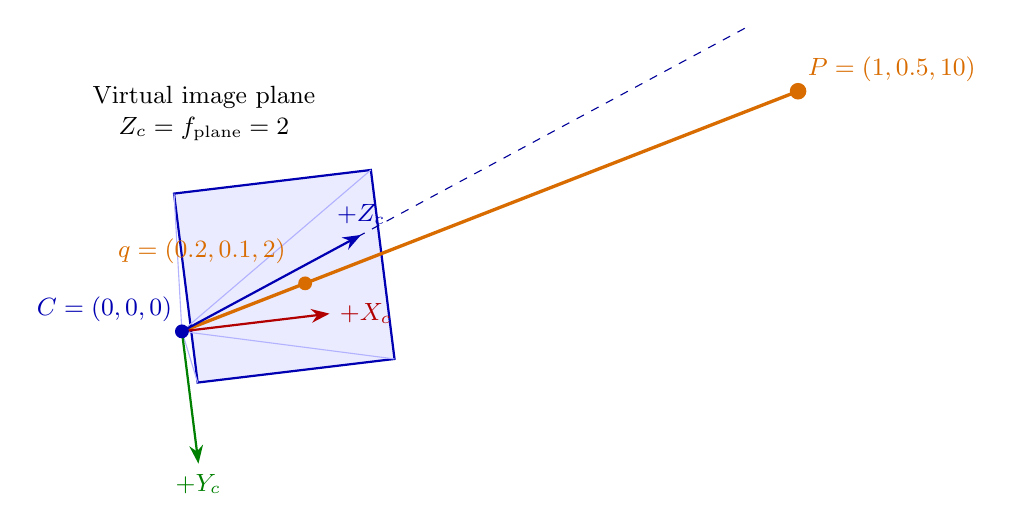
\begin{tikzpicture}[font=\small,arr/.style={-{Stealth},thick},box/.style={draw=blue!55!black,rounded corners,fill=blue!4,align=center,text width=2.9cm,minimum height=1.05cm}]

\begin{scope}[x={(1.25cm,.15cm)},y={(.15cm,-1.2cm)},z={(.65cm,.35cm)}]
\coordinate (C) at (0,0,0);\coordinate (P) at (1,.5,10);\coordinate (Q) at (.2,.1,2);
\fill[blue!12,opacity=.65] (-1,-1,2)--(1,-1,2)--(1,1,2)--(-1,1,2)--cycle;
\draw[blue!70!black,thick] (-1,-1,2)--(1,-1,2)--(1,1,2)--(-1,1,2)--cycle;
\draw[blue!30] (C)--(-1,-1,2) (C)--(1,-1,2) (C)--(1,1,2) (C)--(-1,1,2);
\draw[dashed,blue!60!black] (C)--(0,0,11);
\draw[orange!85!black,very thick] (C)--(P);
\draw[arr,red!70!black] (C)--(1.5,0,0) node[right]{$+X_c$};
\draw[arr,green!50!black] (C)--(0,1.4,0) node[below]{$+Y_c$};
\draw[arr,blue!70!black] (C)--(0,0,3.5) node[above]{$+Z_c$};
\fill[blue!70!black] (C) circle(2.5pt) node[above left]{$C=(0,0,0)$};
\fill[orange!85!black] (P) circle(3pt) node[above right]{$P=(1,0.5,10)$};
\fill[orange!85!black] (Q) circle(2.5pt) node[above left=5pt]{$q=(0.2,0.1,2)$};
\node[align=center] at (-.6,-1.8,2){Virtual image plane\\$Z_c=f_{\rm plane}=2$};
\end{scope}

\end{tikzpicture}
\end{document}
